\subsubsection{Configure GBTx DB to use external \itwoc adapter}
A FFC breakout board is needed to connect \itwoc adapter to the DCB GBTx master.
Follow \autoref{fig:dcb_mc_i2c} to connect an external \itwoc adapter.

\begin{figure}[!ht]
\centering
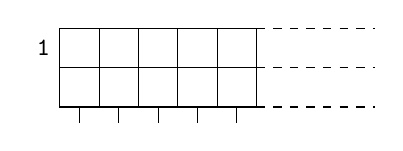
\begin{tikzpicture}
    % Pins
    \draw (0,0) rectangle (0.5,0.5);
    \draw (0.5,0) rectangle (1,0.5);
    \draw (1,0) rectangle (1.5,0.5);
    \draw (1.5,0) rectangle (2,0.5);
    \draw (2,0) rectangle (2.5,0.5);

    \draw (0,-0.5) rectangle (0.5,0);
    \draw (0.5,-0.5) rectangle (1,0);
    \draw (1,-0.5) rectangle (1.5,0);
    \draw (1.5,-0.5) rectangle (2,0);
    \draw (2,-0.5) rectangle (2.5,0);

    % Extension lines
    \draw [dashed] (2.5,0.5) -- (4,0.5);
    \draw [dashed] (2.5,0) -- (4,0);
    \draw [dashed] (2.5,-0.5) -- (4,-0.5);

    % Additional copper traces
    \draw (0.25,-0.5) -- (0.25,-0.7);
    \draw (0.75,-0.5) -- (0.75,-0.7);
    \draw (1.25,-0.5) -- (1.25,-0.7);
    \draw (1.75,-0.5) -- (1.75,-0.7);
    \draw (2.25,-0.5) -- (2.25,-0.7);

    % Helper labels (imaginary)
    \coordinate (B) at (0,0.25);
    \node at (B) [left] {\small\texttt{1}};

    % Single cable on the I2C
    %\draw [black,fill] (0.25,0.25) circle [radius=0.1];
    %\draw [thick] (0.25,0.25)
        %to [out=10,in=190] (5,-1) node [right]
        %{To single cable};

    %% 2x1 connector on the I2C
    %\draw [black,fill] (0.25,-0.25) circle [radius=0.1];
    %\draw [black,fill] (0.75,-0.25) circle [radius=0.1];
    %\draw [thick] (0.25,-0.25) to [out=-80,in=120] (1,-1);
    %\draw [thick] (0.75,-0.25) to [out=-90,in=130] (1,-1);
    %\draw [thick] (1,-1)
        %to [out=-50,in=170] (5,-2) node [right]
        %{To 2x1 connector};
\end{tikzpicture}
\caption{Schematic for external \itwoc adapter setup.}
\label{fig:dcb_mc_i2c}
\end{figure}
